\subsubsection{Espaço de trabalho e cinemática do manipulador}
Como já mencionado, o ambiente de simulação foi desenvolvido utilizando a
arquitetura de planejamento Openrave. Para cada manipulador selecionado após a
pesquisa de mercado, serão analisados os reais espaços de trabalho, e o processo de
revestimento da pá em um ambiente simulado que representa as principais
caracterísiticas do ambiente real.

Para gerar o espaço de trabalho, o Openrave utiliza um método de força bruta,
onde são executadas iterações sob iterações de todas as juntas, por seus ângulos
limites e com o passo de ângulo dependendo da resolução do manipulador. O grau
de manipulabilidade do robô é representado por cores, cujo grau varia do azul
claro (menor manipulabilidade) ao vermelho escuro (maior manipulabilidade).
Entende-se por manipulabilidade a capacidade que o robô possui de manipular
objetos em direções específicas, isto é, em uma posição variadas orientações. Em
todas as simulações, a pistola foi representada como um cilindro de comprimento
300 mm e raio 50 mm, e o efetuador está no extremo do cilindro.

A superfície da pá é amostrada, formando uma grade de tamanho fixo. A técnica
\textit{axis-aligned bounding box (AABB)} é utilizada para obter os
pontos e suas respectivas normais, na superfície da pá. Nesta técnica, a
superfície alvo é inscrita em um bloco, que é uniformemente amostrado. É, então,
realizada uma verificação de colisão entre o ponto amostrado no bloco e a
superfície alvo e, caso haja interseção, o ponto é armazenado, junto com sua
normal à superfície. Dessa forma, podemos amostrar a pá e deslocar os
estes pontos 230 mm em relação à sua normal com a superfície, garantindo a
requerimento do revestimento. A representação dos pontos amostrados e deslocados
em relação às normais da pá podem estão nas figuras~\ref{fig::amostrapa1} e
~\ref{fig::amostrapa2}. 

Utilizando as informações dos pontos amostrados e o espaço de trabalho do
manipulador, foram gerados scripts para calcular a
melhor distância do manipulador em relação a pá, de forma que o maior número de
pontos revestidos fossem cobertos.

\begin{figure}[h!]	
	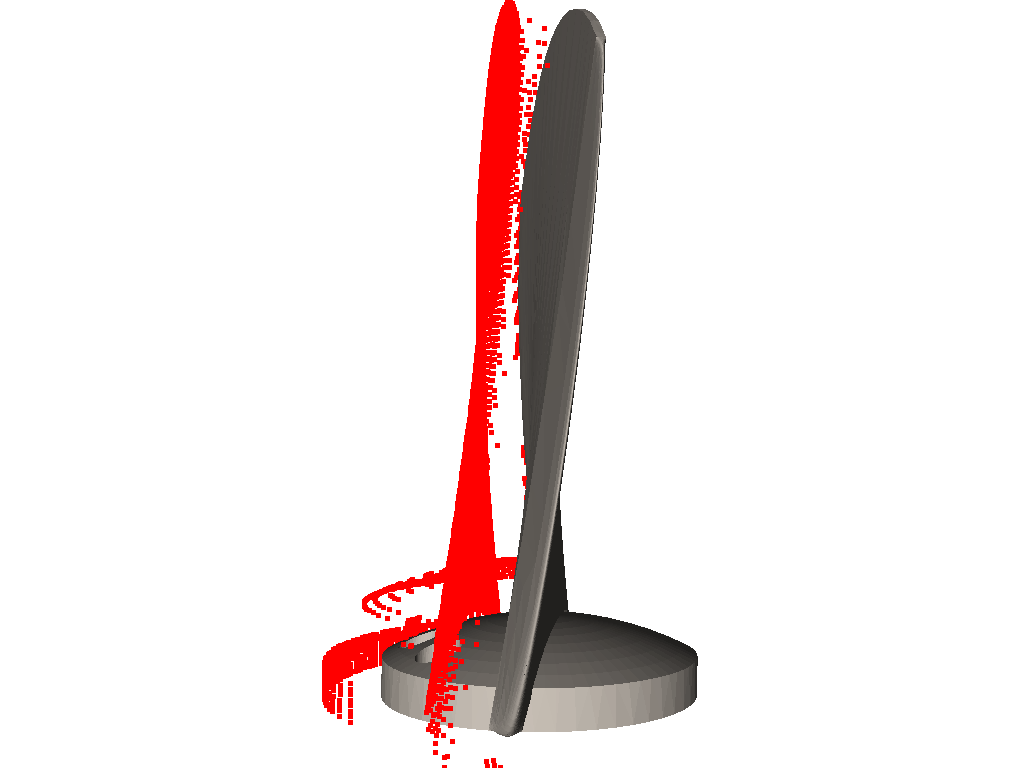
\includegraphics[width=\columnwidth]{figs/bighatch/amostrapa1.png}
	\caption{Pontos amostrados da pá - vista lateral}
	\label{fig::amostrapa1}
\end{figure}

\begin{figure}[h!]	
	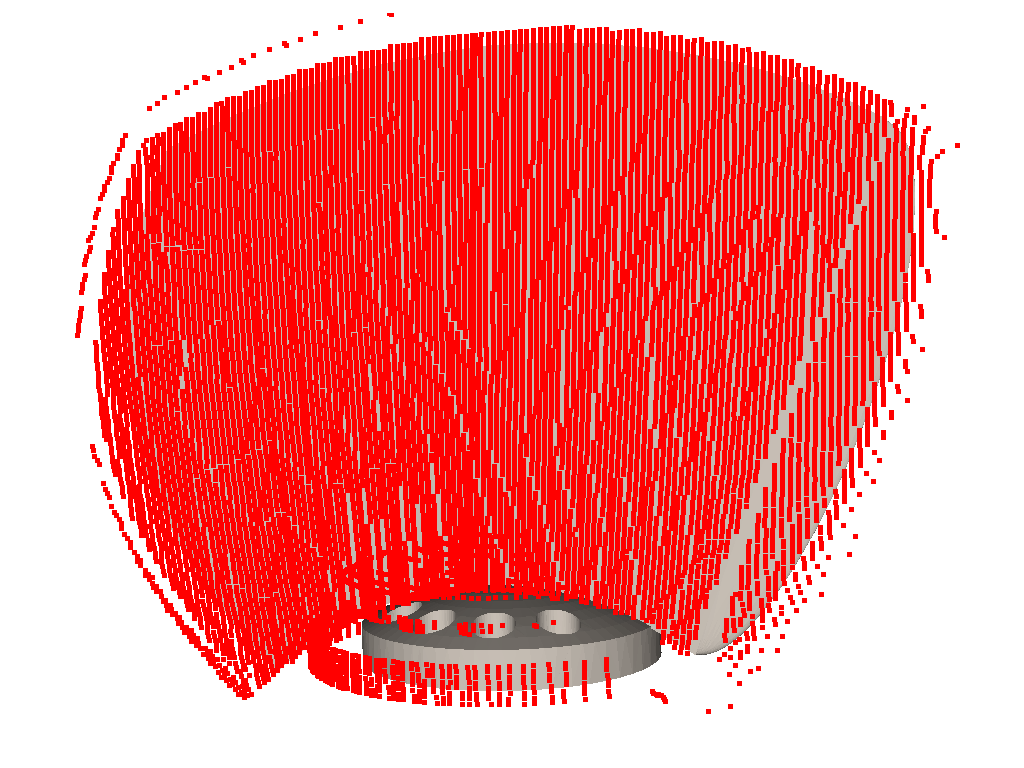
\includegraphics[width=\columnwidth]{figs/bighatch/amostrapa2.png}
	\caption{Pontos amostrados da pá - vista frontal}
	\label{fig::amostrapa1}
\end{figure}

\paragraph{KR 10 R1100 sixx WP (Kuka)}
A figura~\ref{fig::kr10cin1} e figura~\ref{fig::kr10cin2} mostram as vistas
lateral e superior do espaço de trabalho do manipulador, respectivamente.

Um script foi gerado para calcular a melhor distância do manipulador em relação
a pá para que o manipulador faça o revestimento do maior número possíveis de
pontos.

\begin{figure}[h!]	
	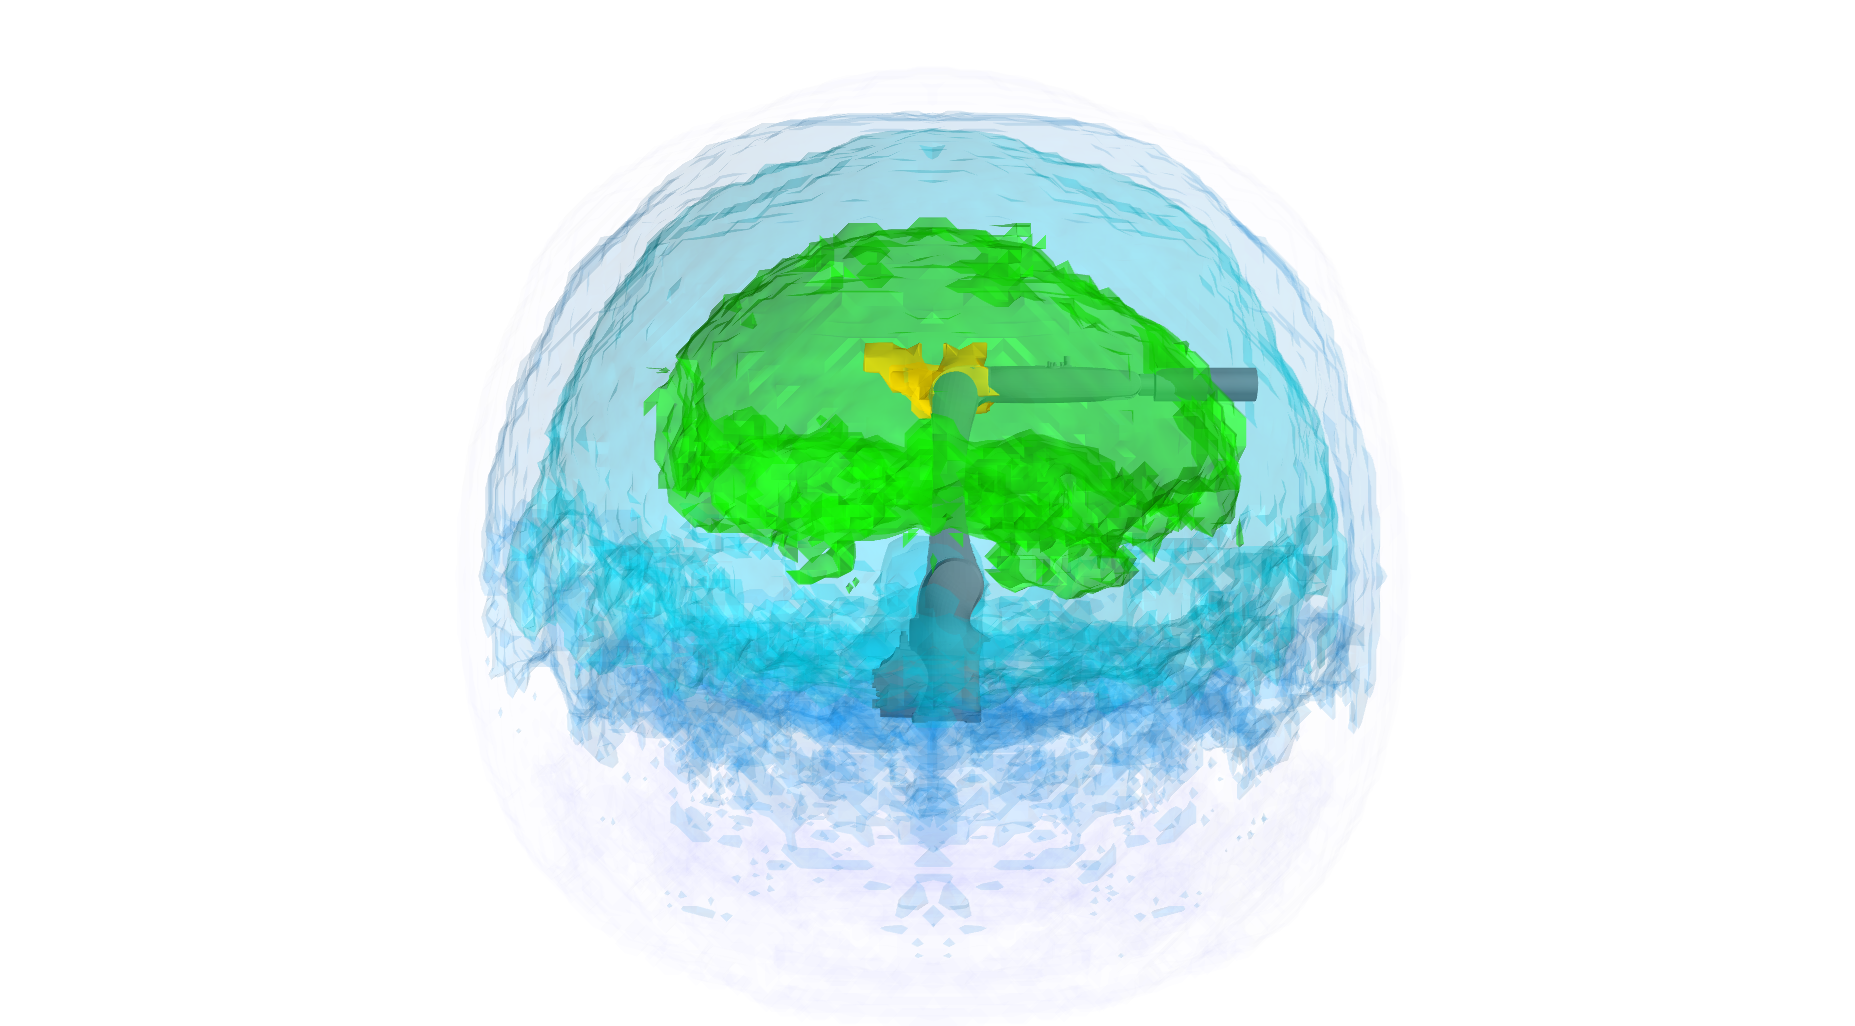
\includegraphics[width=\columnwidth]{figs/bighatch/kr10_front.png}
	\caption{Espaço de trabalho do manipulador Kuka KR10 - vista lateral}
	\label{fig::kr10cin1}
\end{figure}

\begin{figure}[h!]	
	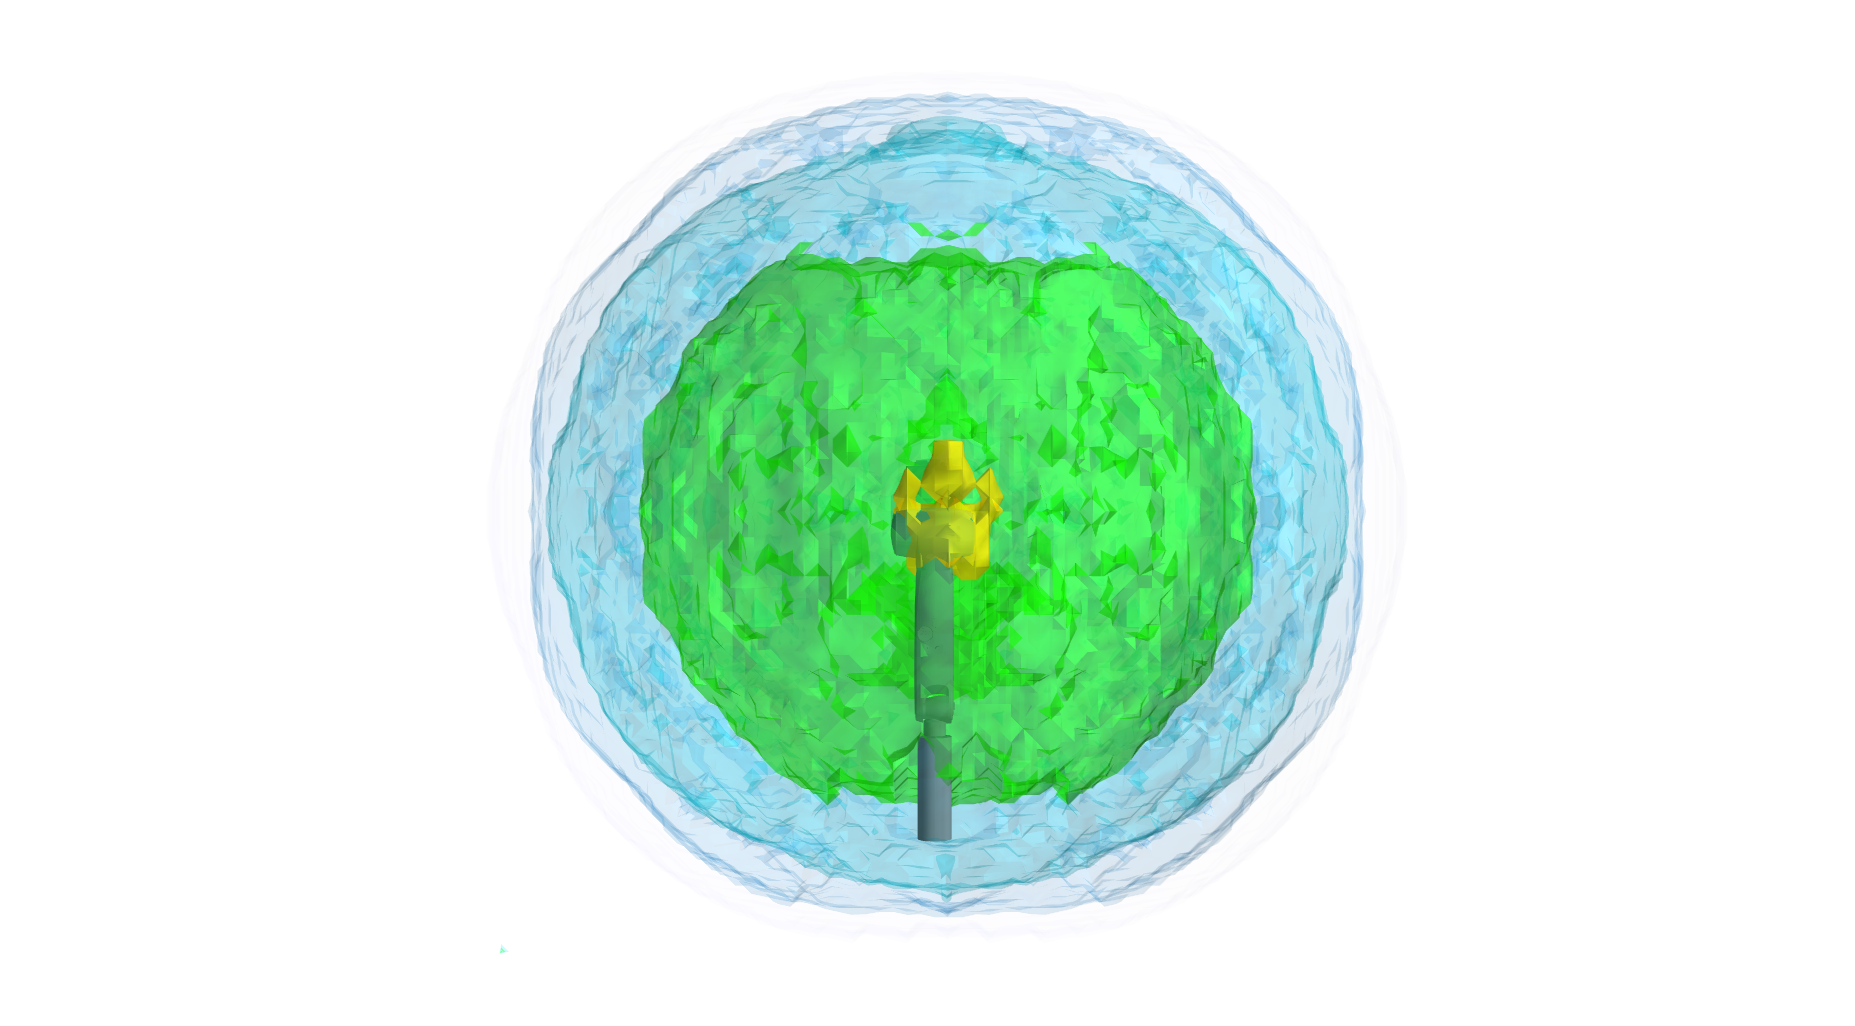
\includegraphics[width=\columnwidth]{figs/bighatch/kr10_top.png}
	\caption{Espaço de trabalho do manipulador Kuka KR10 - vista superior}
	\label{fig::kr10cin2}
\end{figure}




\paragraph{MH12 (Motoman)}



\paragraph{LBR iiwa 14 R820 (Kuka)}
